% Compile with:
% pdflatex main.tex
% bibtex main
% pdflatex main.tex
% pdflatex main.tex
\documentclass[letterpaper]{article}
\usepackage[submission]{aaai2027}
\usepackage[hyphens]{url}
\usepackage{graphicx}
\urlstyle{rm}
\def\UrlFont{\rm}
\usepackage{natbib}
\usepackage{caption}
\frenchspacing

\usepackage{amsmath}
\usepackage{amssymb}
\usepackage{amsthm}
\usepackage{mathtools}
\usepackage{booktabs}
\usepackage{multirow}
\usepackage{tikz}
\usepackage{pgfplots}

\pdfinfo{
/TemplateVersion (2027.1)
}

\usetikzlibrary{arrows.meta,backgrounds,calc,fit,positioning,shapes.geometric}
\pgfplotsset{compat=1.18}

\definecolor{algblue}{RGB}{48,93,145}
\definecolor{detgray}{RGB}{235,237,240}
\definecolor{genfill}{RGB}{225,235,247}
\definecolor{pedfill}{RGB}{247,237,218}
\definecolor{gatefill}{RGB}{245,245,245}
\definecolor{directred}{RGB}{165,61,61}

\newtheorem{definition}{Definition}
\newtheorem{theorem}{Theorem}
\newtheorem{proposition}{Proposition}

\newcommand{\system}{\textsc{AlgoTutorGen}}
\newcommand{\machineok}{\textsc{Machine OK}}
\newcommand{\traceir}{\textsc{SemanticTrace}}
\newcommand{\scenegraph}{\textsc{SceneGraph}}
\newcommand{\runtime}{\textsc{Web Runtime}}
\newcommand{\localresume}{\textsc{Local Resume}}
\newcommand{\globalrestart}{\textsc{Global Restart}}

\setcounter{secnumdepth}{0}

\begin{document}

\title{AlgoTutorGen: Contract-Guided Compositional Synthesis of Verifiable Interactive Algorithm Tutors}
\author{Anonymous Submission}
\affiliations{}

\maketitle

\begin{abstract}
LLM-generated algorithm tutors can display a correct answer while encoding an incorrect trace, unreachable controls, broken feedback, or teaching actions that mutate algorithm state. We call this coupling of heterogeneous obligations in one unconstrained HTML output \emph{constraint entanglement}. \system{} applies contract-guided semantic factorization: an executable specification yields a validated trace and scene, deterministic compilation supplies the runtime, and a separate overlay handles teaching. We characterize two conditional properties, compositional semantic preservation and pedagogical noninterference, and distinguish them from finite implementation evidence. On 200 tasks from 23 algorithm families, \system{} achieves 198/200 complete \machineok{} pages versus 98/200 for Direct HTML, although both display the expected answer on 200/200 pages. Across 294 artifacts, all 55,108 evaluated Trace--SceneGraph--Runtime frames preserve canonical semantic projections. The contracts reject 2,198/2,198 tested semantic violations and accept 392/392 semantics-preserving transformations. A browser stress suite executes 1,561,298 actions over 240 pages without finding a pedagogical noninterference counterexample. \localresume{} nevertheless shows no significant advantage over \globalrestart{} because repair redoes materialization and teaching. Thus semantic and verification decoupling are realized, while full computational recovery decoupling remains open. We make no claim about student learning outcomes. Project page: \url{https://algenlab.github.io/AlgoTutorGen/}.
\end{abstract}

\section{Introduction}
\label{sec:introduction}

Large language models (LLMs) can produce an algorithm-teaching webpage that looks complete and displays the expected answer. That surface success is a weak proxy for an executable tutor. The page may encode an incorrect intermediate state, fail to load, expose controls that cannot be reached, return the same message for correct and incorrect answers, omit a hint or learning log, or let a pedagogical action corrupt the algorithm state. This distinction is visible in our main evaluation: \system{} and a Direct HTML baseline both display the expected answer on 200/200 pages, but only 198/200 and 98/200 pages, respectively, satisfy the full browser-level \machineok{} conjunction. The difficult part is therefore not answer text alone; it is the simultaneous construction of an algorithm execution, its visual representation, a working browser program, and a stateful teaching interaction.

We diagnose this failure mode as \emph{constraint entanglement}. A monolithic generator must satisfy answer, trace, scene, runtime, feedback, and noninterference obligations in one open-ended artifact:
\[
\begin{aligned}
&C_{\mathrm{answer}},\ C_{\mathrm{trace}},\ C_{\mathrm{scene}},\\
&C_{\mathrm{runtime}},\ C_{\mathrm{feedback}},\ C_{\mathrm{noninterference}}.
\end{aligned}
\]
These obligations are implemented by the same HTML, JavaScript, data literals, and event handlers. A repair intended to make a button work can overwrite a correct answer; a visual rewrite can desynchronize a pointer; and adding feedback can mutate the execution frame. More generation budget does not by itself remove such cross-obligation interference.

\system{} addresses this problem with \emph{contract-guided semantic factorization}. An LLM first produces an executable solution specification. Sandboxed materialization records a typed \traceir{} through a restricted tracing interface. Validators check the result, trace structure, process continuity, and scene bindings. A deterministic compiler maps the verified trace to a \scenegraph{}, and a fixed \runtime{} renders it. A separately constrained pedagogical overlay may change explanations, hints, prediction feedback, and learning-log state, but not the canonical algorithmic projection. A final browser audit checks the released page. The chain converts an opaque generation problem into explicit refinement obligations, where failures can be rejected at the boundary that exposes them.

This factorization supports two forms of reasoning. First, if the trace-to-scene and scene-to-runtime projections agree at every reachable frame, semantic preservation follows by transitivity. Second, if pure pedagogical actions leave algorithm state unchanged and navigation selects only verified frames, arbitrary finite interaction sequences preserve a runtime invariant. These are conditional statements about the abstract contracts, not a machine-assisted proof that every source trace is correct. We connect each premise to executable checks and state the remaining assumptions. We also analyze an ideal stage-local recovery policy, but the current implementation does not satisfy its full checkpointability premise.

The evidence follows the same separation. On a paired 200-task, 23-family benchmark, \system{} improves \machineok{} by 50.0 percentage points over Direct HTML (95\% paired-bootstrap confidence interval (CI) [43.0, 57.0], exact McNemar $p=4.06\times10^{-29}$). All 55,108 evaluated representation frames agree under the canonical projection; all 2,198 tested semantic mutations are rejected while all 392 tested semantics-preserving transformations are accepted; and no noninterference counterexample is found in 1,561,298 browser actions. Cross-model and held-out experiments retain the reliability gap. By contrast, the recovery experiment is negative: retaining a solution specification does not produce a significant success advantage over restarting, because materialization and teaching are recomputed.

Our contributions are: \textbf{(1)} formulating interactive tutor generation as constraint-entangled artifact synthesis; \textbf{(2)} a contract-guided factorization separating generated semantics, deterministic compilation, browser execution, and teaching state; \textbf{(3)} conditional preservation and noninterference results plus the assumptions for ideal local recovery; and \textbf{(4)} evaluation of executable reliability, contract survival, semantic discrimination, noninterference, model variation, held-out tasks, ablations, scalability, and the negative recovery result.

\section{Problem Formulation}
\label{sec:problem}

This section defines the synthesized artifact and the obligations that distinguish an executable tutor from a page containing a correct answer.

\subsection{Inputs, Artifacts, and Contracts}

An input is $x=(q,i,e,c)$: algorithmic problem $q$, concrete instance $i$, optional oracle $e$, and optional reference code or strategy $c$. The internal synthesis bundle is $A=(S,T,G,P,R)$, comprising executable specification $S$, \traceir{} $T$, \scenegraph{} sequence $G$, pedagogical overlay $P$, and browser runtime $R$. Deterministic export turns $A$ into the released webpage $W$.

We require the conjunction
\begin{align}
\Phi(A,W,x)={}&\Phi_{\mathrm{result}}\land\Phi_{\mathrm{trace}}
\land\Phi_{\mathrm{scene}}\land\Phi_{\mathrm{runtime}}\nonumber\\
&\land\Phi_{\mathrm{feedback}}
\land\Phi_{\mathrm{noninterference}}.
\label{eq:global-contract}
\end{align}
$\Phi_{\mathrm{result}}$ compares the computed result with $e$ when an oracle is available. $\Phi_{\mathrm{trace}}$ checks the typed event sequence, final-state consistency, and generic causal or state-continuity conditions. $\Phi_{\mathrm{scene}}$ checks that visual objects, marks, pointers, edges, and frames bind to trace entities. $\Phi_{\mathrm{runtime}}$ covers loading and reachability. $\Phi_{\mathrm{feedback}}$ requires distinguishable correct and incorrect responses plus hint, answer, and log behavior. $\Phi_{\mathrm{noninterference}}$ requires the teaching layer to be read-only with respect to algorithm facts, except that navigation may select another verified frame.

\subsection{Monolithic and Factored Search}

Direct HTML asks a model to construct a point in an open space $\Omega_{\mathrm{HTML}}$ whose textual answer, embedded data, rendering logic, event handlers, and teaching state jointly satisfy Equation~\eqref{eq:global-contract}. A defect is often observable only after a browser executes the whole artifact, and a whole-file rewrite can invalidate an obligation that was previously satisfied.

\system{} instead constructs a refinement chain
\[
\begin{aligned}
S &\xRightarrow{C_S} T
\xRightarrow{C_T} G
\xRightarrow{C_G} R,\\
G &\xrightarrow{\text{teaching}} P
\xRightarrow{C_P} \bar P,\\
(R,\bar P)&\xRightarrow{C_B} W,
\end{aligned}
\]
where each $C$ is an executable contract at a representation boundary. This notation does not claim that writing the output space as a Cartesian product automatically reduces search complexity. The benefit comes from four operational choices: contracts reject invalid candidates before release; verified semantic data are reused rather than regenerated; deterministic stages remove open-ended choices from downstream code; and failures are attributed to a narrower boundary. Modularization without these properties would merely rearrange the same entanglement.

\section{System Design}
\label{sec:system}

This section explains how \system{} assigns one semantic responsibility to each intermediate representation and where the implementation remains less modular than the idealized architecture.

\begin{figure*}[t]
\centering
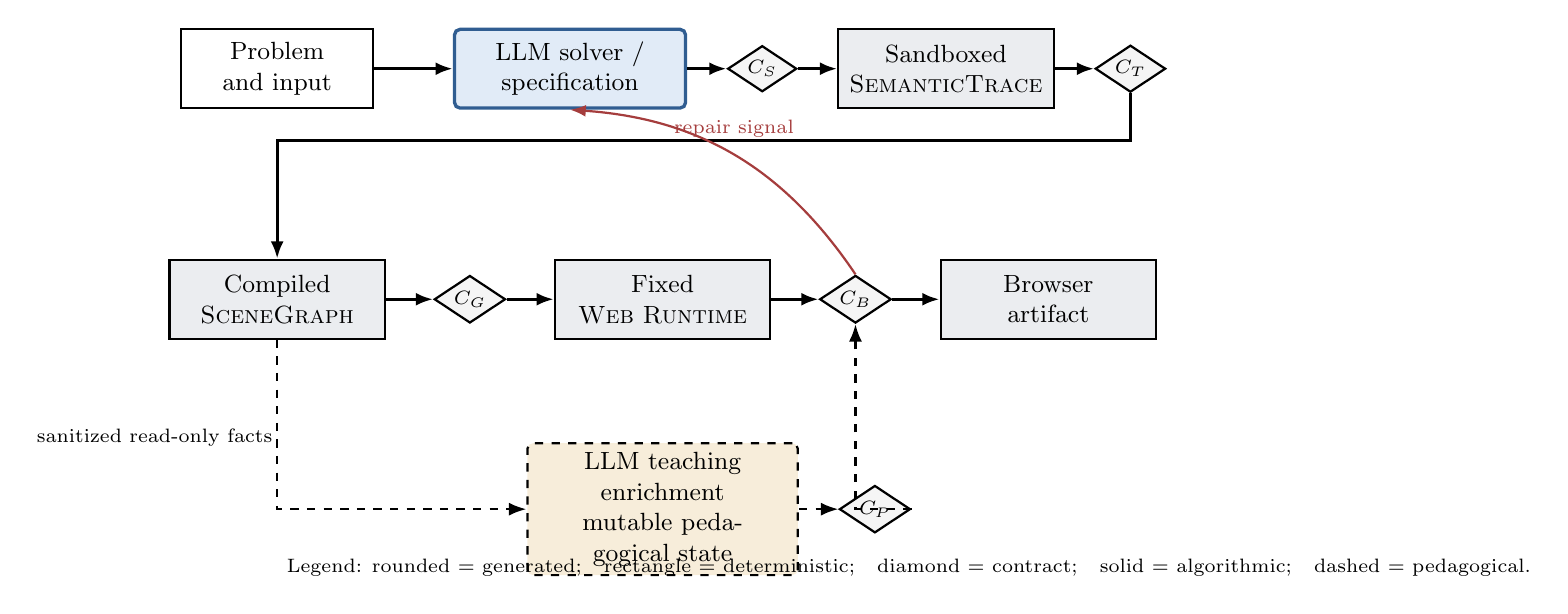
\begin{tikzpicture}[
  font=\small,
  node distance=6mm,
  alg/.style={draw=algblue, very thick, rounded corners=2pt, fill=genfill,
    minimum height=10mm, text width=27mm, align=center},
  det/.style={draw=black, thick, fill=detgray,
    minimum height=10mm, text width=25mm, align=center},
  input/.style={draw=black, thick, minimum height=10mm, text width=22mm, align=center},
  gate/.style={diamond, draw=black, thick, fill=gatefill, aspect=1.5,
    inner sep=1.1pt, align=center, font=\scriptsize},
  ped/.style={draw=black, thick, dashed, rounded corners=2pt, fill=pedfill,
    minimum height=10mm, text width=32mm, align=center},
  flow/.style={-{Latex[length=2.2mm]}, very thick},
  pflow/.style={-{Latex[length=2.2mm]}, thick, dashed},
  note/.style={font=\scriptsize, align=center}
]
\node[input] (input) {Problem\\and input};
\node[alg, right=10mm of input] (spec) {LLM solver / specification};
\node[gate, right=5mm of spec] (sc) {$C_S$};
\node[det, right=5mm of sc] (trace) {Sandboxed\\\traceir{}};
\node[gate, right=5mm of trace] (tc) {$C_T$};

\node[det, below=19mm of input] (scene) {Compiled\\\scenegraph{}};
\node[gate, right=6mm of scene] (gc) {$C_G$};
\node[det, right=6mm of gc] (runtime) {Fixed\\\runtime{}};
\node[gate, right=6mm of runtime] (bc) {$C_B$};
\node[det, right=6mm of bc] (page) {Browser\\artifact};

\draw[flow] (input) -- (spec);
\draw[flow] (spec) -- (sc);
\draw[flow] (sc) -- (trace);
\draw[flow] (trace) -- (tc);
\draw[flow] (tc.south) -- ++(0,-6mm) -| (scene.north);
\draw[flow] (scene) -- (gc);
\draw[flow] (gc) -- (runtime);
\draw[flow] (runtime) -- (bc);
\draw[flow] (bc) -- (page);

\node[ped, below=13mm of runtime] (teach) {LLM teaching enrichment\\mutable pedagogical state};
\node[gate, right=5mm of teach] (pc) {$C_P$};
\draw[pflow] (scene.south) |- node[note, near start, below left=-1mm] {sanitized read-only facts} (teach.west);
\draw[pflow] (teach) -- (pc);
\draw[pflow] (pc.east) -| (bc.south);

\node[note, below=29mm of scene, anchor=west] (legend) {Legend: rounded = generated;\quad rectangle = deterministic;\quad diamond = contract;\quad solid = algorithmic;\quad dashed = pedagogical.};

\draw[-{Latex[length=2mm]}, bend right=26, thick, directred]
  (bc.north) to node[note, above=1mm, text=directred] {repair signal} (spec.south);
\end{tikzpicture}
\caption{\system{} architecture. Rounded blue boxes are open-ended LLM stages; rectangular gray boxes are deterministic stages; diamonds are executable contracts. Solid flow carries canonical algorithmic state. Dashed flow carries mutable pedagogical state derived from a sanitized, read-only view. The repair loop shown is the implemented specification-level boundary, not a fully checkpointed retry at every stage.}
\label{fig:architecture}
\end{figure*}

The open-ended stage emits an executable solution specification that solves the instance and records events through \texttt{TraceSession}. A sandbox restricts imports, time, serialization, and communication. Materialization produces typed snapshots containing stable identifiers, values, marks, pointers, graph edges, containers, steps, and final answers, but no CSS or event handlers. Result and trace validators check oracle agreement, schema, and internal consistency. The process validator checks generic DSL causality and continuity; it is not a proved operational semantics for all 23 families, so stronger source-trace claims still require family or human audit.

A deterministic compiler binds trace objects to scene cells, nodes, edges, pointers, highlights, queues, stacks, and annotations. The online scene validator checks schema, nonempty frames, object-ID uniqueness, visible objects, and the integrity of mark, parent, source, and target references. Canonical Trace--SceneGraph--Runtime projection agreement is measured separately by the offline preservation audit; it is not part of this structural scene gate. The shared \runtime{} supplies layout, navigation, variants, and rendering in a self-contained page. Teaching enrichment receives sanitized verified facts and may change objectives, explanations, predictions, hints, answer reveals, and logs, but fields redefining algorithm state are removed or rejected. The browser release audit checks the nine \machineok{} conditions. On failure, \localresume{} retains the specification but reruns materialization and teaching; it is not five-stage checkpoint recovery (Section~\ref{sec:recovery}).

\section{Theoretical Analysis}
\label{sec:theory}

This section states what follows from the representation contracts. The results are paper-and-pencil implications of explicit premises. They are not claims of machine-checked verification for arbitrary generated traces.

\subsection{Canonical Algorithmic Projection}

\begin{definition}[Canonical algorithmic projection]
\label{def:projection}
Let $\mathcal{A}$ be a representation-independent algorithm-state space containing stable object identifiers, values, marks, pointers, graph edges, stack or queue contents, the current step, and the final answer. For trace frame $T_t$, scene frame $G_t$, and reachable runtime state $R_t$, define
\[
 \alpha_T:T_t\rightarrow\mathcal{A},\qquad
 \alpha_G:G_t\rightarrow\mathcal{A},\qquad
 \alpha_R:R_t\rightarrow\mathcal{A}.
\]
Layout coordinates, CSS, explanatory prose, hint visibility, prediction text, and learning-log contents are excluded from $\mathcal{A}$.
\end{definition}

The implementation serializes these projections in a canonical order before comparison and hashing. An equality therefore means equality of normalized algorithm facts, not pixel equality.

\subsection{Compositional Semantic Preservation}

\begin{theorem}[Compositional Semantic Preservation]
\label{thm:preservation}
For input $x$, let $S(x)$ be a verified solver result, let
$T=(T_0,\ldots,T_n)$ be a semantic trace, let
$G=(G_0,\ldots,G_n)$ be its compiled scene sequence, and let $R(G)$ be the rendered runtime execution. Suppose
\begin{align*}
\operatorname{Final}(T)&=S(x),\\
\alpha_T(T_t)&=\alpha_G(G_t) &&\text{for every }t,\\
\alpha_G(G_t)&=\alpha_R(R_t) &&\text{for reachable }t.
\end{align*}
Then $\alpha_T(T_t)=\alpha_R(R_t)$ for every reachable $t$, and the rendered final answer equals $S(x)$. If additionally $S(x)=\operatorname{Oracle}(x)$, the rendered final answer equals the oracle.
\end{theorem}

\begin{proof}
Transitivity gives $\alpha_T(T_t)=\alpha_R(R_t)$ at each reachable $t$. At the final frame its answer component is $\operatorname{Final}(T)=S(x)$; substituting oracle equality proves the last claim.
\end{proof}

Theorem~\ref{thm:preservation} is a layer-to-layer preservation theorem. It does not establish that an arbitrary $T$ is the intended stepwise algorithm. The result and trace checks support $\operatorname{Final}(T)=S(x)$, and the projection audit checks the two representation equalities on finite artifacts. Correctness of every source event relative to an independent algorithm semantics remains an assumed or separately audited premise.

\subsection{Pedagogical Noninterference}

We adapt the noninterference idea of separating protected and observable state~\cite{Goguen1982Noninterference} to a user-interface setting. Let runtime state be $\sigma=(a,p)$, where $a\in\mathcal{A}$ is algorithmic state and $p$ is pedagogical state. Pure pedagogical actions are \path{submit_correct}, \path{submit_wrong}, \path{hint}, \path{show_answer}, and \path{clear_learning_log}. Navigation uses \path{next}, \path{previous}, and \path{timeline}; it also includes \path{reset} and \path{select_variant}.

\begin{theorem}[Pedagogical Noninterference]
\label{thm:noninterference}
Suppose every pure pedagogical action $u$ satisfies
\[
  \delta_u(a,p)=(a,p')
\]
for some $p'$. Then, for every finite sequence of pure pedagogical actions $u_1,\ldots,u_m$,
\[
\pi_A\!\left(\delta_{u_m}\circ\cdots\circ\delta_{u_1}(a,p)\right)=a.
\]
Moreover, if each navigation action selects an algorithm state from the verified trajectory
\[
\mathcal{V}(T)=\{\alpha_T(T_0),\ldots,\alpha_T(T_n)\},
\]
then after any finite mixed sequence of pure pedagogical and navigation actions, the algorithm state belongs to $\mathcal{V}(T)$.
\end{theorem}

\begin{proof}
Induct on sequence length. A pure action preserves $a$; a navigation action replaces the current member of $\mathcal{V}(T)$ with another member. Each induction step therefore preserves the corresponding invariant.
\end{proof}

The theorem describes the intended abstract runtime. The concrete browser stress test checks for violations of its premises through state, step, and artifact hashes; passing finite tests is not a proof for all future code or action sequences.

\subsection{Nested Contract Survival}

\begin{proposition}[Nested contract survival]
\label{prop:survival}
For sequential contract events $C_1,\ldots,C_m$ with nonzero conditioning probabilities,
\[
\Pr\!\left(\bigcap_{i=1}^{m}C_i\right)
=\prod_{i=1}^{m}
\Pr\!\left(C_i\mid \bigcap_{j=1}^{i-1}C_j\right).
\]
\end{proposition}

This is the probability chain rule, not a new result. Its diagnostic value is that cumulative survival localizes the first lossy boundary. Figure~\ref{fig:survival} shows large monolithic losses at runtime, interaction, and feedback, while factored survival stays near one after semantic validation.

\subsection{Conditional Stage-Local Recovery}

\begin{theorem}[Ideal stage-local recovery]
\label{thm:recovery}
Consider $k$ sequential stages with cost $c_i>0$ and independent, stationary per-attempt success probability $p_i\in(0,1]$. Suppose a validator identifies the failing stage exactly; every successful stage is checkpointable; a failed stage can be retried independently; retry does not invalidate prior stages; and verified downstream work is not recomputed. Then
\[
\mathbb{E}[C_{\mathrm{local}}]=\sum_{i=1}^{k}\frac{c_i}{p_i},
\qquad
\mathbb{E}[C_{\mathrm{global}}]
=\sum_{i=1}^{k}\frac{c_i}{\prod_{j=i}^{k}p_j},
\]
and $\mathbb{E}[C_{\mathrm{local}}]\leq
\mathbb{E}[C_{\mathrm{global}}]$.
\end{theorem}

\begin{proof}
Geometric retry yields local multiplicity $1/p_i$ and global multiplicity $1/\prod_{j=i}^{k}p_j$. Summation gives both costs; $\prod_{j=i}^{k}p_j\leq p_i$ proves the inequality.
\end{proof}

This theorem is a conditional characterization, not a performance guarantee for the current system. Repairing a solution specification triggers materialization and teaching again, violating full checkpointability and the no-recomputation premise. The negative experiment in Section~\ref{sec:recovery} is therefore a test of the implementation boundary, not a contradiction of Theorem~\ref{thm:recovery}.

\section{Experimental Setup}
\label{sec:setup}

This section defines the evaluation protocol and the meaning of each reported metric.

\subsection{Tasks and Generation Conditions}

The benchmark contains 200 tasks from 23 algorithm families and 646 concrete samples. The paired main comparison uses sample index 0 for each task, avoiding overweighting tasks that have more stored samples. The original main \system{} condition uses DeepSeek-V4-Pro. Cross-model final-quality experiments use DeepSeek-V4-Flash, GLM-5.2, and Kimi-K2.5. They begin with two candidates and two repair rounds; failed tasks may receive a recorded final-quality retry of at most three candidates and three rounds. The reported cross-model table uses the resulting frozen pages and is therefore not a uniform-call or token-matched comparison. A frozen held-out set contains 40 new cases from 15 families.

The Direct HTML prompt receives the problem, concrete input, and expected answer, and explicitly requests a complete self-contained teaching page with timeline, correct and incorrect feedback, hint, answer reveal, and learning log. Thus it is not denied the oracle or teaching requirements. Both approaches may use their specified repair policy. The main table uses selected-final artifacts after allowed retries: \system{} initially generated 195/200 primary pages and filled five missing artifacts with recorded targeted retries. Direct generated all selected pages within its allowed calls. This boundary prevents interpreting 200 available pages as first-pass generation success.

WebGen-Agent and strict Direct-plus-HTMLCure are external code paths adapted to the same browser audit. Their numbers measure performance under this task and audit protocol, not a reproduction of the authors' original benchmark claims. External network resources are blocked during final evaluation so a page must be self-contained.

\subsection{Metrics and Statistical Tests}

\machineok{} conjoins page load, visible-answer match, reachable interaction, correct feedback, wrong feedback, hint, answer reveal, learning log, and a lightweight answer-protection check. The ninth check compares the protected visible-answer summary before and after the audited teaching actions; the stronger algorithm-state, step, and artifact-hash comparison is reported separately in the noninterference stress test. We report exact counts; paired binary differences use exact two-sided McNemar tests, percentage-point differences use paired bootstrap CIs, and test families use Holm correction. Secondary paired scores use Wilcoxon tests where applicable. None measures student learning.

\subsection{Theory-Aligned Audits}

The preservation audit compares normalized $\alpha_T$, $\alpha_G$, and $\alpha_R$ for every frame in 200 main artifacts, a completed 40-artifact held-out set, and 54 long-trace artifacts. The mutation audit injects semantic violations and semantics-preserving changes. The determinism audit recompiles and rerenders 20 artifacts ten times each. The noninterference audit runs 100 random mixed action sequences on each of 240 pages and compares algorithm-state, step, and artifact hashes after every action.

The held-out generation experiment originally produced 39/40 valid \system{} artifacts. A targeted retry later supplied the fortieth artifact only for preservation and noninterference coverage. We keep 39/40 as the generation result and label the 40/40 collection as a completed audit set.

\section{Results}
\label{sec:results}

We organize the results by the obligation being tested: complete executable reliability, survival through nested contracts, representation-level semantics, interaction isolation, and robustness to model or task variation.

\subsection{RQ1: Does Factorization Improve Executable Reliability?}

\begin{table*}[t]
\centering
\caption{Main 200-task browser reliability. Every entry is a count out of 200. \machineok{} is the conjunction of nine checks, including the five displayed component columns and hint, answer reveal, learning log, and protected-answer stability.}
\label{tab:main-reliability}
\small
\begin{tabular}{lrrrrrr}
\toprule
Method & Load & \shortstack{Visible\\answer} & \shortstack{Interaction\\reachable} &
\shortstack{Correct\\feedback} & \shortstack{Wrong\\feedback} & \machineok{} \\
\midrule
\system{} & 200 & 200 & 200 & 199 & 198 & \textbf{198} \\
Direct HTML & 188 & 200 & 149 & 120 & 125 & 98 \\
WebGen-Agent & 194 & 169 & 154 & 74 & 89 & 45 \\
Direct + HTMLCure (strict) & 75 & 75 & 62 & 52 & 51 & 40 \\
\bottomrule
\end{tabular}
\end{table*}

Table~\ref{tab:main-reliability} shows that answer visibility alone saturates for both principal methods, but full behavior does not. \system{} reaches 198/200 (99.0\%) \machineok{} versus 98/200 (49.0\%) for Direct HTML, a paired difference of 50.0 percentage points (95\% CI [43.0, 57.0]). There are 101 pairs where only \system{} passes, one where only Direct passes, and 98 concordant pairs; exact McNemar $p=4.06\times10^{-29}$. The difference is concentrated in executable interaction and feedback rather than the displayed result.

The external paths obtain 45/200 and 40/200 under the same strict conjunction. Their failure profiles differ: WebGen-Agent usually loads but often misses answer or feedback requirements, whereas the strict HTMLCure path loses many pages before full interaction evaluation. These results support a protocol-specific comparison of released artifacts, not a universal ranking of website-generation systems.

\subsection{RQ2: Where Do Monolithic Artifacts Fail?}

\begin{figure}[t]
\centering
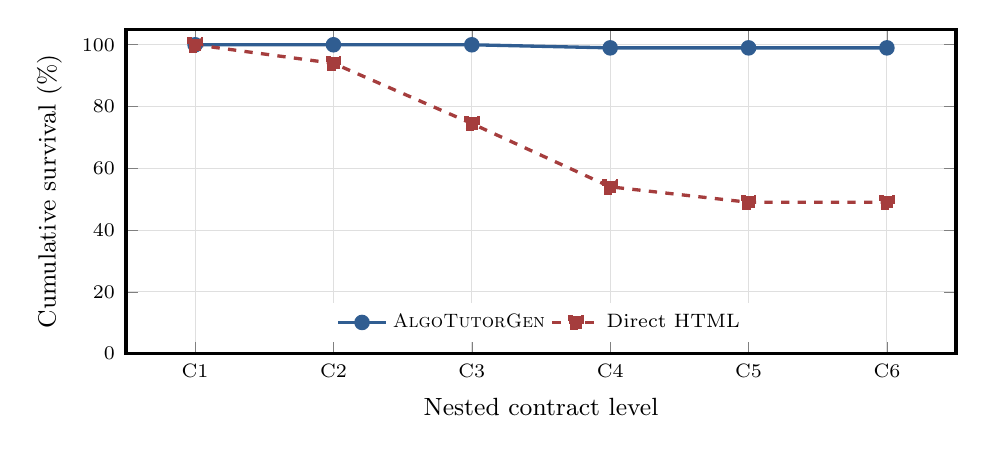
\begin{tikzpicture}
\begin{axis}[
  width=\columnwidth,
  height=5.7cm,
  ymin=0,
  ymax=105,
  ytick={0,20,40,60,80,100},
  ylabel={Cumulative survival (\%)},
  symbolic x coords={C1,C2,C3,C4,C5,C6},
  xtick=data,
  xlabel={Nested contract level},
  grid=major,
  grid style={draw=gray!25},
  tick label style={font=\scriptsize},
  label style={font=\small},
  legend style={font=\scriptsize, at={(0.5,0.03)}, anchor=south,
    legend columns=2, draw=none, fill=white},
  line width=1.2pt,
  mark size=2.2pt
]
\addplot[color=algblue, mark=*, solid]
  coordinates {(C1,100) (C2,100) (C3,100) (C4,99) (C5,99) (C6,99)};
\addlegendentry{\system{}}
\addplot[color=directred, mark=square*, dashed]
  coordinates {(C1,100) (C2,94) (C3,74.5) (C4,54) (C5,49) (C6,49)};
\addlegendentry{Direct HTML}
\end{axis}
\end{tikzpicture}
\caption{Nested contract survival on the main benchmark. C1: answer; C2: load; C3: reachable interaction; C4: bidirectional feedback; C5: hint, answer reveal, and log; C6: protected-answer stability. Values are cumulative, not independent per-contract accuracies; full-state noninterference is audited separately.}
\label{fig:survival}
\end{figure}

Figure~\ref{fig:survival} applies Proposition~\ref{prop:survival}. \system{} remains at 100\% through interaction and loses two pages at feedback, after which the surviving set remains stable. Direct HTML drops from 100\% answer match to 94.0\% load, 74.5\% interaction, 54.0\% bidirectional feedback, and 49.0\% complete teaching support. The same qualitative pattern appears under Flash, GLM, and Kimi: the factored pipeline retains high downstream survival, while Direct loses additional artifacts at interaction and feedback boundaries. This evidence localizes constraint entanglement; it does not imply independence among contracts.

\begin{figure*}[t]
\centering
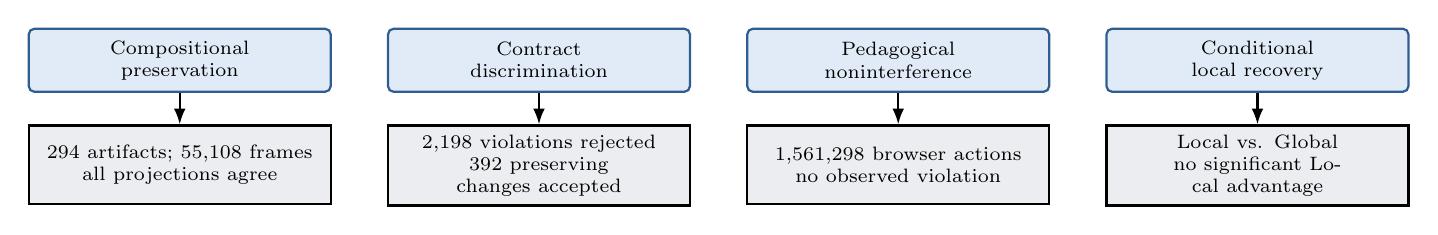
\begin{tikzpicture}[
  font=\scriptsize,
  prop/.style={draw=algblue, thick, rounded corners=2pt, fill=genfill,
    text width=36mm, minimum height=8mm, align=center},
  evidence/.style={draw=black, thick, fill=detgray,
    text width=36mm, minimum height=10mm, align=center},
  arr/.style={-{Latex[length=2mm]}, thick}
]
\node[prop] (p1) {Compositional\\preservation};
\node[prop, right=7mm of p1] (p2) {Contract\\discrimination};
\node[prop, right=7mm of p2] (p3) {Pedagogical\\noninterference};
\node[prop, right=7mm of p3] (p4) {Conditional\\local recovery};

\node[evidence, below=4mm of p1] (e1) {294 artifacts; 55,108 frames\\all projections agree};
\node[evidence, below=4mm of p2] (e2) {2,198 violations rejected\\392 preserving changes accepted};
\node[evidence, below=4mm of p3] (e3) {1,561,298 browser actions\\no observed violation};
\node[evidence, below=4mm of p4] (e4) {Local vs. Global\\no significant Local advantage};

\draw[arr] (p1) -- (e1);
\draw[arr] (p2) -- (e2);
\draw[arr] (p3) -- (e3);
\draw[arr] (p4) -- (e4);
\end{tikzpicture}
\caption{Theory-to-evidence map. Projection equality does not prove source-trace correctness; mutation and browser results cover finite suites; recovery is negative because checkpointability is absent.}
\label{fig:theory-evidence}
\end{figure*}

\subsection{RQ3: Are Semantics Preserved and Contracts Discriminative?}

\begin{table*}[t]
\centering
\caption{Theory-aligned executable evidence. The rightmost column states the strongest warranted interpretation.}
\label{tab:theory-evidence}
\scriptsize
\begin{tabular}{@{}p{0.20\textwidth}p{0.22\textwidth}p{0.52\textwidth}@{}}
\toprule
Property and scope & Observed outcome & Evidence boundary \\
\midrule
Projection, 294 artifacts & 55,108/55,108 frames agree &
Representation preservation on evaluated frames; source-trace correctness is a separate premise. \\
Determinism, 20 artifacts $\times$ 10 & One projection and render hash per artifact &
Stable in the tested environment, not a cross-platform bitwise claim. \\
Semantic violations & 2,198/2,198 rejected &
Complete for defined mutation operators, not universal validator soundness. \\
Preserving transformations & 392/392 accepted &
Complete for 195 teaching rewrites, 195 visual-metadata changes, and two equivalent reorderings. \\
Noninterference, 240 pages & 1,561,298 actions; zero violations &
No counterexample in 24,000 sequences, not proof of every execution. \\
\bottomrule
\end{tabular}
\end{table*}

The main, completed held-out, and long-trace sets contribute 9,421, 4,568, and 41,119 agreeing frames, respectively. This supports Theorem~\ref{thm:preservation}'s representation premises but does not prove that every source event is the intended algorithm step. The mutation suite rejects all 2,198 defined semantic violations and accepts all 392 preserving transformations (195 teaching rewrites, 195 visual-metadata changes, and two equivalent reorderings). We call this \emph{contract discrimination} on the defined suite, not universal soundness and completeness. Twenty artifacts also produce one projection and render hash each across ten reruns.

\subsection{RQ4: Does the Concrete Runtime Respect Teaching Isolation?}

The suite executes 24,000 random sequences and 1,561,298 actions on 240 pages: 435,859 pure pedagogical actions preserve algorithm state, step, and artifact hash, while 1,125,439 navigation actions land on verified frames. All overlays pass sanitization; illegal algorithm fields are removed or rejected. No counterexample is found, but finite randomized execution does not establish noninterference for all future code.

\subsection{RQ5: Does the Reliability Gap Persist?}

\begin{table*}[t]
\centering
\caption{Cross-model final-quality and frozen held-out \machineok{} results. Cross-model rows use 200 paired tasks; \system{} starts from a two-candidate, two-repair budget and applies recorded final-quality retries to failed tasks, so calls and tokens are not matched to Direct. The held-out row uses 40 new cases.}
\label{tab:cross-model}
\small
\begin{tabular}{lrrrrr}
\toprule
Model or set & \system{} & Direct & Difference & 95\% paired-bootstrap CI & Exact McNemar $p$ \\
\midrule
DeepSeek-V4-Flash & 200/200 (100.0\%) & 118/200 (59.0\%) & +41.0 pp & [34.5, 48.0] & $4.14\times10^{-25}$ \\
GLM-5.2 & 196/200 (98.0\%) & 35/200 (17.5\%) & +80.5 pp & [75.0, 86.0] & $2.81\times10^{-47}$ \\
Kimi-K2.5 & 194/200 (97.0\%) & 87/200 (43.5\%) & +53.5 pp & [46.0, 60.5] & $4.79\times10^{-30}$ \\
Held-out, 15 families & 39/40 (97.5\%) & 18/40 (45.0\%) & +52.5 pp & [37.5, 67.5] & $9.54\times10^{-7}$ \\
\bottomrule
\end{tabular}
\end{table*}

% Conflict resolution: the original held-out generation result is 39/40.
% A later targeted retry supplied the 40th artifact only for semantic audits.
Table~\ref{tab:cross-model} shows positive paired differences for each model and the held-out set; varying absolute success reflects strict gate rejection, model variation, and the recorded final-quality retry policy, not model invariance or equal compute. On held-out tasks, Direct generates 40/40 self-contained pages but only 18 pass, whereas \system{} produces 39 valid pages and all pass. A later targeted completion supplies audit coverage only and does not change the original 39/40 result.

\subsection{Ablation Summary}

Two 50-task ablations isolate the representation boundaries. Replacing executable tracing with Direct-to-SceneGraph reduces \machineok{} from 49/50 to 1/50; replacing deterministic compilation with free HTML from a verified trace reduces it from 49/50 to 0/50 despite 50/50 visible answers. Neither a fixed runtime nor a correct trace alone is sufficient.

\section{Negative Result: Recovery Is Not Yet Decoupled}
\label{sec:recovery}

This section tests whether the implementation meets the checkpoint premise of Theorem~\ref{thm:recovery}. The result is negative and materially changes the system claim.

\begin{table*}[t]
\centering
\caption{\localresume{} versus \globalrestart{} on paired 50-task sets. Tokens and time are normalized by successful pages. The McNemar value compares success within each model; nonsignificance is not evidence of equivalence.}
\label{tab:recovery}
\small
\begin{tabular}{llrrrr}
\toprule
Model & Strategy & Success & Tokens/success & Mean time to valid & Exact McNemar $p$ \\
\midrule
\multirow{2}{*}{DeepSeek-V4-Flash}
 & \localresume{} & 38/50 (76.0\%) & 71,369 & 172.9 s & \multirow{2}{*}{0.4545} \\
 & \globalrestart{} & 42/50 (84.0\%) & 62,256 & 194.2 s & \\
\addlinespace
\multirow{2}{*}{GLM-5.2}
 & \localresume{} & 42/50 (84.0\%) & 92,385 & 533.8 s & \multirow{2}{*}{1.0000} \\
 & \globalrestart{} & 43/50 (86.0\%) & 96,186 & 558.2 s & \\
\bottomrule
\end{tabular}
\end{table*}

For Flash, \globalrestart{} is numerically better in both success (42/50 versus 38/50) and tokens per success (62,256 versus 71,369), although its mean successful completion time is higher. For GLM, \localresume{} uses slightly fewer tokens and less time per successful page, but succeeds on one fewer task. Neither paired success comparison is significant. We therefore find no evidence that the implemented Local policy improves success, and no consistent cost advantage.

Instrumentation explains the mismatch between the ideal theorem and the measured system. Local repair reduces solution-specification generation and repair work, but the repaired specification is materialized again and teaching enrichment is invoked again. Those calls can dominate or erase the saved work. In addition, a locally repaired candidate may preserve a specification that is less amenable to downstream teaching than a fresh global draw. The implementation provides specification-level repair, not independently checkpointed solver, trace, scene, runtime, and teaching stages.

The result does not contradict Theorem~\ref{thm:recovery}; it shows that its strongest premises are absent. More importantly, it distinguishes three concepts that are easy to conflate. \system{} substantially realizes \emph{semantic decoupling} and \emph{verification decoupling}. It does not yet realize full \emph{computational recovery decoupling}. Semantic factorization is therefore necessary infrastructure for local recovery, but it does not automatically supply computational checkpointing.

\section{Related Work}
\label{sec:related}

\paragraph{Generated webpages and educational visualization.}
Design2Code and WebGen-Bench evaluate front-end reconstruction or functional website generation~\cite{Si2025Design2Code,Lu2025WebGenBench}; WebGen-Agent and HTMLCure add iterative browser feedback and repair~\cite{Lu2025WebGenAgent,HTMLCure2026}, while EduVisAgent studies pedagogical-visualization planning~\cite{Ji2025EduVisAgent}. Our task is narrower, but each page is compiled from an executable trace and audited for cross-representation state and teaching isolation; external-baseline results therefore apply only to our protocol.

Algorithm-visualization work distinguishes passive viewing from active engagement and cautions that visualization alone does not ensure learning~\cite{Naps2002Engagement,Hundhausen2002MetaStudy}. TRAKLA2, Python Tutor, JSAV, OpenDSA, VisuAlgo, JHAVE, and Algorithm Visualizer provide assessed exercises, execution views, libraries, or curated content~\cite{Malmi2004TRAKLA2,Guo2013PythonTutor,Karavirta2013JSAV,Shaffer2011OpenDSA,Halim2015VisuAlgo,Naps2005JHAVE,AlgorithmVisualizer2026}; surveys characterize this broader design space~\cite{Sorva2013ProgramVisualization}. These systems generally use human-authored algorithms or templates, whereas \system{} synthesizes benchmark-task artifacts. Multimedia learning, LORI, and visualization-validation principles inform interface analysis~\cite{Mayer2009MultimediaLearning,Leacock2007LORI,Munzner2009NestedModel}, but do not justify a learning-gain claim here.

\paragraph{Synthesis, contracts, and testing.}
Program synthesis and systems such as Sketch and SYNQUID use explicit specifications to constrain search~\cite{Gulwani2017ProgramSynthesis,SolarLezama2006Sketch,Polikarpova2016Synquid}. Interface automata and modular temporal reasoning expose component assumptions~\cite{deAlfaro2001InterfaceAutomata,Pnueli1985ModularReasoning}; CompCert proves compiler preservation mechanically~\cite{Leroy2009CompCert}. In contrast, our preservation theorem is conditional and its implementation evidence is finite. We borrow state separation from noninterference~\cite{Goguen1982Noninterference} and counterexample search from QuickCheck and metamorphic testing~\cite{Claessen2000QuickCheck,Segura2016Metamorphic}, without claiming an information-flow proof.

\section{Discussion and Limitations}
\label{sec:discussion}

Factorization works because intermediate representations expose comparable semantic objects, contracts reject defects early, deterministic compilation reuses verified facts, and teaching receives a sanitized read-only view. The ablations show that neither a fixed runtime without executable semantics nor a verified trace followed by free HTML is sufficient; reliability comes from the complete refinement chain.

Mathematically, Theorems~\ref{thm:preservation} and~\ref{thm:noninterference} establish conditional refinement and state invariants, while Theorem~\ref{thm:recovery} assumes ideal checkpointing. Experimentally, all evaluated projections agree, the defined mutation suite discriminates violations from preserving changes, and no noninterference counterexample appears in 1,561,298 actions. These results do not prove arbitrary source traces correct, establish universal validator guarantees, or ensure future browser executions are safe. The recovery result adds a systems lesson: semantic factorization does not automatically imply computational checkpointing. Future recovery should persist versioned stage artifacts and invalidate only descendants of changed semantic objects.

\machineok{} measures executable completeness, not teaching quality or learning, and may favor the fixed runtime. Two-annotator calibration of 120 pages and an independent 40-task trace audit remain unlabeled. Mutation operators and action sequences are finite; the main study uses one sample per task, the 646-sample replay is unbalanced and contains failures, and held-out evaluation has 40 cases. Compute also differs: selected-final \system{} averages 5.33 calls and 76.8k tokens per task versus 1.11 calls and 21.9k for Direct, while the fixed runtime embodies additional engineering.

Remote models can drift and external baselines are task-adapted. Full-frame export also scales poorly: large traces average 1,636.7 frames, 160.42 MB, 8.354 s load, 101.3 ms step latency, and 185.6 MB heap; two extremes reach 581 MB and 1.08 GB and exceed 60 s. Delta encoding and virtualization are needed. Stage2 visual ratings use one vision-language evaluator, and expert and 24-student studies remain protocols. No usability, retention, transfer, or learning-gain result is claimed.

\section{Conclusion}
\label{sec:conclusion}

Interactive algorithm tutors are constraint-entangled artifacts: algorithm facts, execution traces, visual states, browser behavior, feedback, and teaching-state isolation must all hold together. \system{} replaces monolithic HTML generation with contract-guided semantic factorization through an executable specification, semantic trace, validated scene, deterministic runtime, and isolated teaching overlay. Under the evaluated protocol, this architecture raises complete browser reliability from 98/200 to 198/200 while preserving canonical projections for all 55,108 evaluated frames and revealing no pedagogical noninterference counterexample in 1.56 million actions. These are strong finite executable results linked to conditional compositional theorems, not formal verification of arbitrary traces or evidence of student learning. The negative recovery experiment sharpens the conclusion: semantic and verification decoupling do not automatically provide computational checkpointing. Building truly stage-local, dependency-aware recovery is the next systems boundary.

\bibliography{references}

\end{document}
